\newpage
\section{Theorie}
\subsection{Grundlagen}
Kriterien für Einteilung Energieversorgungsnetze:
\begin{itemize}
    \item Spannungsart \item Spannungshöhe \item Funktion \item Topologie
\end{itemize}
% - Spannungsart \qquad - Spannungshöhe\\
% - Funktion \qquad \qquad- Topologie

Arten der Netztopologien:
\begin{itemize}
\item Strahlennetz (z.B. Kfz-Bordnetz)
\item Ringnetz
\item Maschennetz
\end{itemize}

Spannungshöhe:
\begin{itemize}
    \item Höchstspannung (HöS) $380/220 \, kV$
    \item Hochspannung (HS) $100 \, kV$
    \item Mittelspannung (MS) $10/20 \, kV$
    \item Niederspannung (NS) $<1 \, kV$
\end{itemize}

Tages-Belastungsdiagramm:
\begin{itemize}
    \item \ul{Grundlast}: Kernenergie, Braunkohle, Laufwasser\\
        produzieren konstant Strom, träge Wärmeprozesse
        \item \ul{Mittellast}: Erdgas, Steinkohle, Heizöl\\
            vorhersehbar schwankender Teil der benötigten Leistung
            \item \ul{Spitzenlast}: Pumpspeicher, Gasturbinen\\
                schnell zuschaltbar, Abdeckung Lastspitzen (bei Mittag, Abend)
\end{itemize}
Residuallast: Netzlast abzüglich fluktierender Einspeiseleistung der erneuerbaren Energien,
entspricht der Last, die konventionelle Kraftwerke abdecken müssen

\subsection{Trafos}
\ul{Kühlungsart}\\
O: Ölisolierung \qquad N: Natürlich durch Auftrieb\\
A: Luft \qquad W: Wasser \qquad F: Fremd durch Lüfterpumpen

Beispiel:\\
ONAN: Ölkreislauf natürlich, Kühler (Radiatoren) natürlich\\
OFWF: Ölkreislauf gepumpt, Wasserkühler mit Pumpen\\

\ul{Schaltgruppen}\\
OS: Y, YN, D \qquad US: y, yn, d, zn, a\\
N/n: mit Sternpunktleiter\\
zn: Zick-Zack (nur Sternpunktschaltung)\\
a: Sparwicklung

Beispiel: Dy5 $\rightarrow$ Dreieck OS, Stern US, $5\cdot 30 \degree = 150\degree$ Phasenversatz zwischen OS/US.

% \subsection{Freileitungen}
\subsection{Kabel}

\ul{Leiterprofile (Aufbau-Kurzzeichen)}\\
R: Rundleiter \qquad O: Ovalleiter \qquad S: Segmentleiter\\
H: Hohlleiter \qquad E: Eindrähtig \qquad M: Mehrdrähtig \\
V: Verdichtet \quad $\rightarrow$ weitere Kurzzeichen: siehe F34

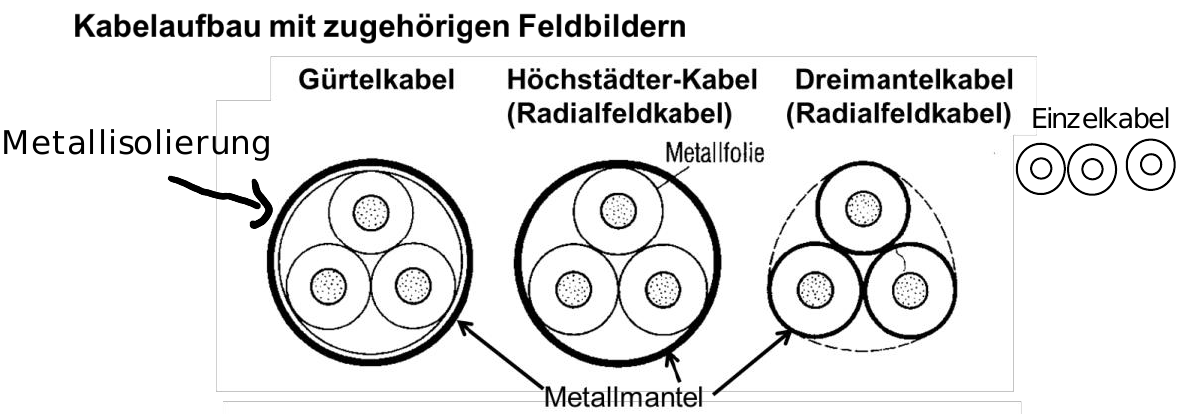
\includegraphics[width=1.0 \columnwidth]{figures/Kabelaufbau.png}

% Feldprobleme an Kabelenden

% Betriebskonstanten:
\begin{center}
\begin{tabular}[h]{l|l|l|}
    & Freileitung & Kabel\\
    \hline
Reaktanzbelag & groß & klein\\
    \hline
Kapazitätsbelag & klein & groß \\
\hline
Wellenwiderstand & groß & klein \\
\hline
Natürliche Leistung & klein & groß
\end{tabular}
\end{center}

\subsection{Generator}

Polradspannung $U_p$: Im Stator induzierte Spannung\\
Polradwinkel $\vartheta$: Winkel Polrad- zu Klemmenspannung

\begin{tabular}[h]{|l|l|l|}
    \hline
    Aufbau & Stator & Rotor\\
    \hline
    Innenpol & Induktionsspule & Permanentmagnet\\
    \hline
    Außenpol & Permanentmagnet & Induktionsspule\\
    \hline
\end{tabular}

$\Rightarrow$ Drehstrom-Synchronmaschinen als Innenpolgenerator!

% \subsubsection{Bauart des Rotors}
% Rotorbauart

\ul{Wirkleistungs-Polradwinkel-Diagramm}
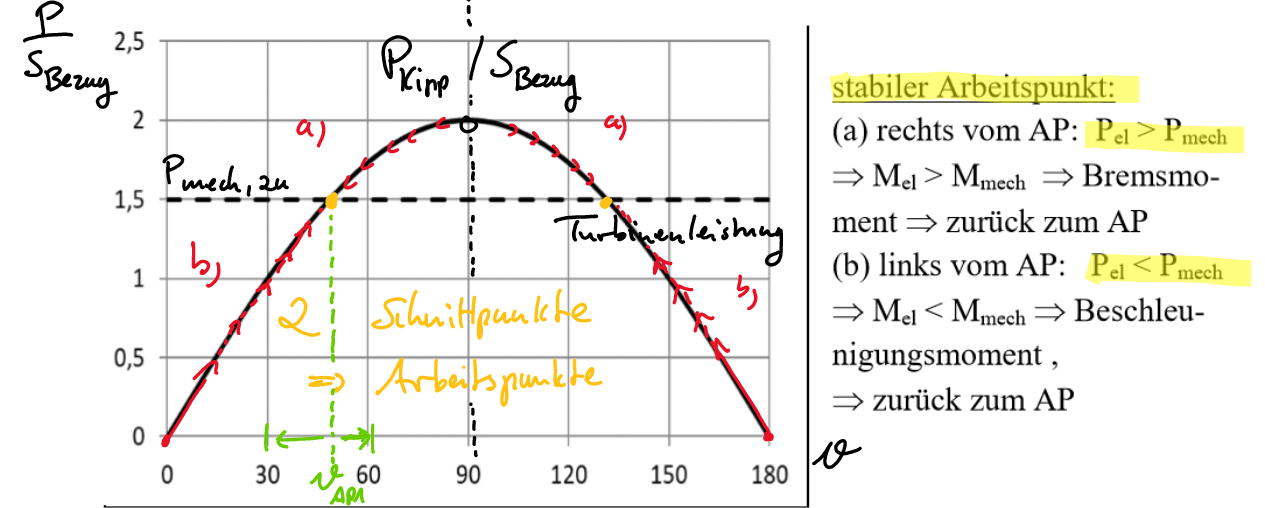
\includegraphics[width=1.0 \columnwidth]{figures/wirkleistungs_diagramm.png}

% \ul{Belastungskennlinie}

\makebox[\columnwidth]
{
\begin{minipage}[c]{0.5\columnwidth}
    \centering
    Belastungskennlinie
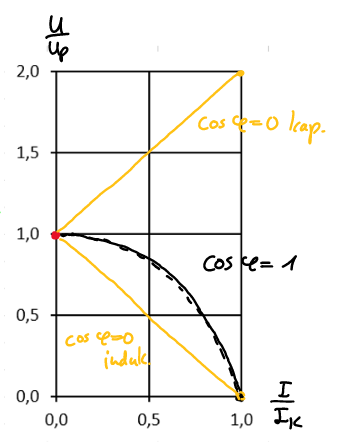
\includegraphics[width=0.7 \columnwidth]{figures/belastungskennlinie_generator.png}
\end{minipage}
\begin{minipage}[c]{0.5\columnwidth}
    \centering
    Regulierkennlinie
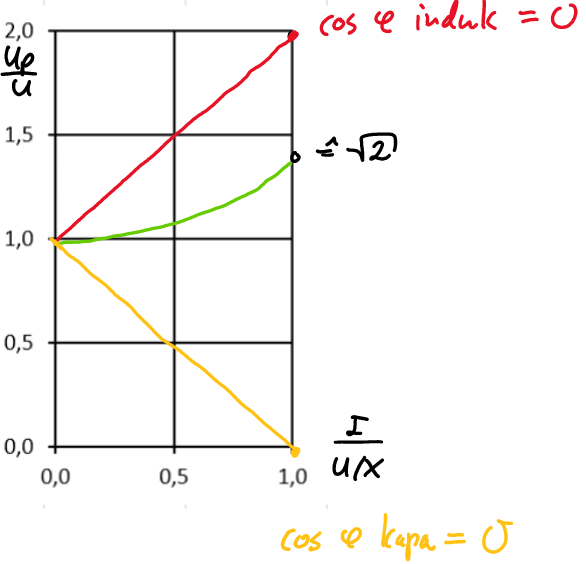
\includegraphics[width=1 \columnwidth]{figures/regulierkennlinie.png}
\end{minipage}
}

\subsection{Schaltgeräte}
Löschen des Lichtbogens (LiBo):
\begin{itemize}
\item Verlängerung des LiBo (thermischer Auftrieb)
\item Kühlung des LiBo (Öl, MS)
\item Aufteilen des LiBo (Löschbleche, in NS)
\end{itemize}
